\chapter{Ley de Ampère. Magnetización de la materia}

\chaptermark{Ley de Ampère}

\begin{miparrafo}
Teorema de Ampère
El físico y matemático André-Marie Ampère (1775-1836) enunció uno de los principales teoremas del electromagnetismo que suele considerarse como el homólogo magnético del teorema de Gauss.

Si recuerdas bien, el campo eléctrico es conservativo lo que implica que su circulación a lo largo de una línea cerrada es nula:

$$ \oint \vec E \cdot \dd \vec l = \nabla V =0$$

Como hemos visto anteriormente, las líneas de campo magnético generado por una corriente rectilínea son circulares y en general, al contrario que las líneas de campo eléctrico o gravitatorio, no tienen comienzo ni final. Sin embargo, los campos magnéticos no son conservativos y por tanto, la circulación a lo largo de una línea cerrada no es nula y viene dada por la ley de Ampère.

La ley de Ampère determina que la circulación del campo magnético a lo largo de una línea cerrada es equivalente a la suma algebraica de las intensidades de la corrientes que atraviesan la superficie delimitada por la línea cerrada, multiplicada por la permitividad del medio. En concreto para el vacío:

$$ \oint \vec B \cdot \dd \vec l = \mu_o \sum I$$

\rightline{\textcolor{gris}{`https://www.fisicalab.com/apartado/ley-de-ampere'}}
\end{miparrafo}

\section{Teorema de la circulación de Amprère}

\begin{multicols}{2}
Supongamos un circuito recorrido por una corriente de intensidad $I$.

En $P$ habrá un campo magnético creado por la corriente.

Vamos a calcular una cantidad llamada \emph{circulación del campo magnético}:
\begin{figure}[H]
	\centering
	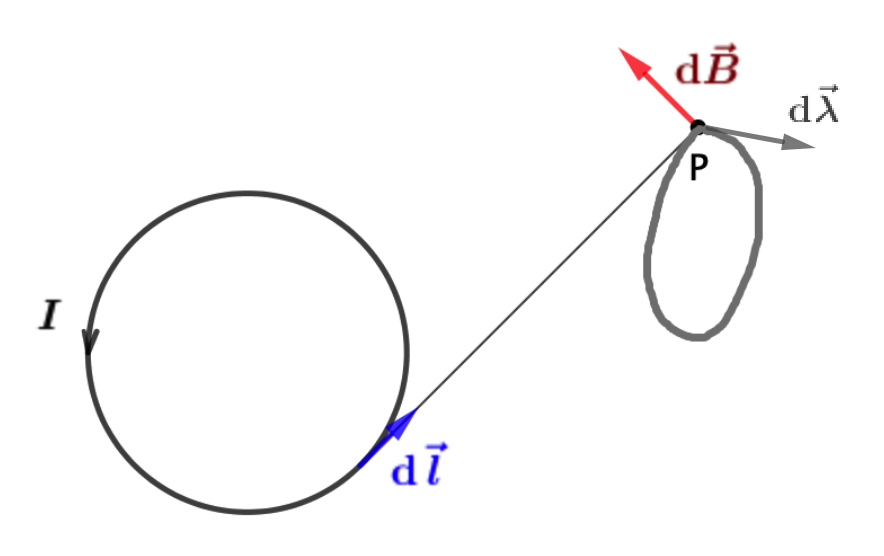
\includegraphics[width=.5\textwidth]{imagenes/imagenes27/T27IM01.png}
\end{figure}	
\end{multicols}
$$\mathcal C_B=\displaystyle \oint_L \vec B \cdot \dd \vec l$$

La circulación puede interpretarse como una medida de la rotación neta del campo a lo largo de la curva.

Supongamos que $P$ se traslada una distancia $\dd \vec \lambda$, podemos calcular $\vec B \cdot \dd \vec \lambda$. Ocurrirá lo mismo que si suponemos que el punto $P$ permanece fijo y es el circuito quien se desplaza $\dd \vec \lambda$ en sentido contrario ($-\dd \vec \lambda$).

Si varia la posición relativa de $P$ respecto al circuito, variará el ángulo sólido del circuito debido a esta variación $\dd \vec \lambda$.

\begin{multicols}{2}
	El ángulo sólido será la suma de los infinitos ángulos sólidos elementales que han hecho variar al circuito los elementos $\dd \vec l$. El valor de estas áreas elementales las da el módulo del producto vectorial: $-\dd \vec \lambda \times  \dd \vec l$. Si proyectamos esta área en la dirección del elemento del circuito $\dd \vec l$ hacia el punto $P$, tendremos: $(-\dd \vec \lambda \times  \dd \vec l)\cdot \vec u_r$ y, finalmente, dividiendo por el cuadrado de la distancia al punto $P,\ r^2$ obtenemos la variación al ángulo sólido con que ha contribuido el elemento de circuito $\dd \vec l$:
\begin{figure}[H]
	\centering
	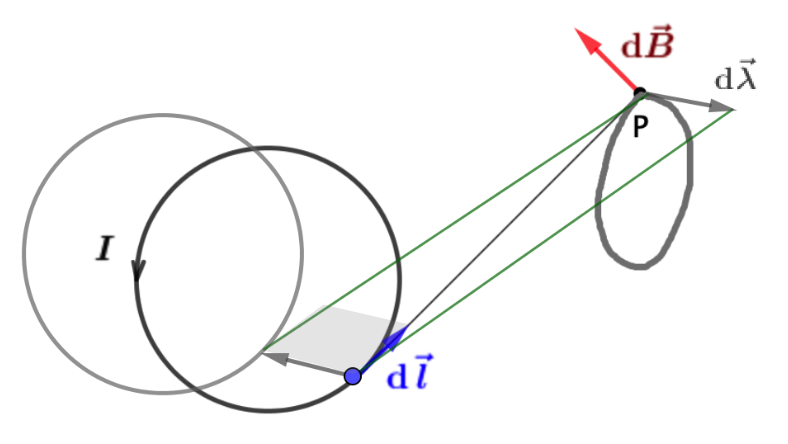
\includegraphics[width=.5\textwidth]{imagenes/imagenes27/T27IM02.png}
\end{figure}
\end{multicols}

$$\displaystyle \mathrm{d}^2 {\Omega}=\dfrac{(-\dd \vec \lambda \times  \dd \vec l)\cdot \vec u_r}{r^2}$$

\textcolor{gris}{Sabemos que el producto mixto de tres vectores se calcula como el determinante de una matriz $3\times 3$ cuyas filas son las componentes de los tres vectores:
$ (\vec a\times \vec b)\cdot \vec c=\left| \begin{matrix} a_x&a_y&a_z 
\\ b_x&b_y&b_z \\ c_x&c_y&c_z \end{matrix} \right|$}

\textcolor{gris}{Si se cambias dos filas de un determinante, éste no varía.}

$$\mathrm{d}^2 \Omega=\dfrac{-\dd \vec \lambda \cdot (\dd \vec l \times \vec u_r)}{r^2}$$

Para calcular la contribución de todo el circuito a la variación total de ángulo sólido visto desde $P$, integraremos. ($\dd \vec \lambda$ es constante para todos los elementos del circuito):
$\quad \displaystyle \dd \Omega =\dd \vec \lambda \cdot \oint_C \dfrac {\dd \vec l \times \vec u_r}{r^2}$

En el tema anterior, vimos la ley de Ampère-Laplace: $\displaystyle B=\dfrac{\mu_0}{4\pi}I\oint_C  \dfrac {\dd \vec l \times \vec u_r}{r^2}$, por lo que, ahora,
$ \quad \displaystyle \dd \Omega =\dd \vec \lambda \cdot \vec B \dfrac{4\pi}{\mu_0 I}$, de donde deducimos que:

$$\vec B \cdot \dd \vec \lambda=-\dfrac{\mu_0 I}{4\pi} \dd \Omega$$

y ya tenemos el integrando de la \emph{circulación}. Teniendo en cuenta que $\displaystyle \oint \dd \Omega=\Delta \Omega $,

\begin{equation}
\subrayado{ \ \boxed{ \ \boldsymbol{\oint_L \vec B \cdot \dd \vec l \ = \ -\dfrac{\mu_0\ I}{4\ \pi} \ \Delta \Omega } \ } \ } \qquad \textbf{Teorema Ampère circulación} 
\end{equation}

La circulación de un campo magnético en un circuito es directamente proporcional a la intensidad y a la variación de ángulo sólido.

\subsection{Casos particulares del teorema de Ampère}

Estudiaremos la variación de ángulo sólido en dos casos: 

\begin{figure}[H]
	\centering
	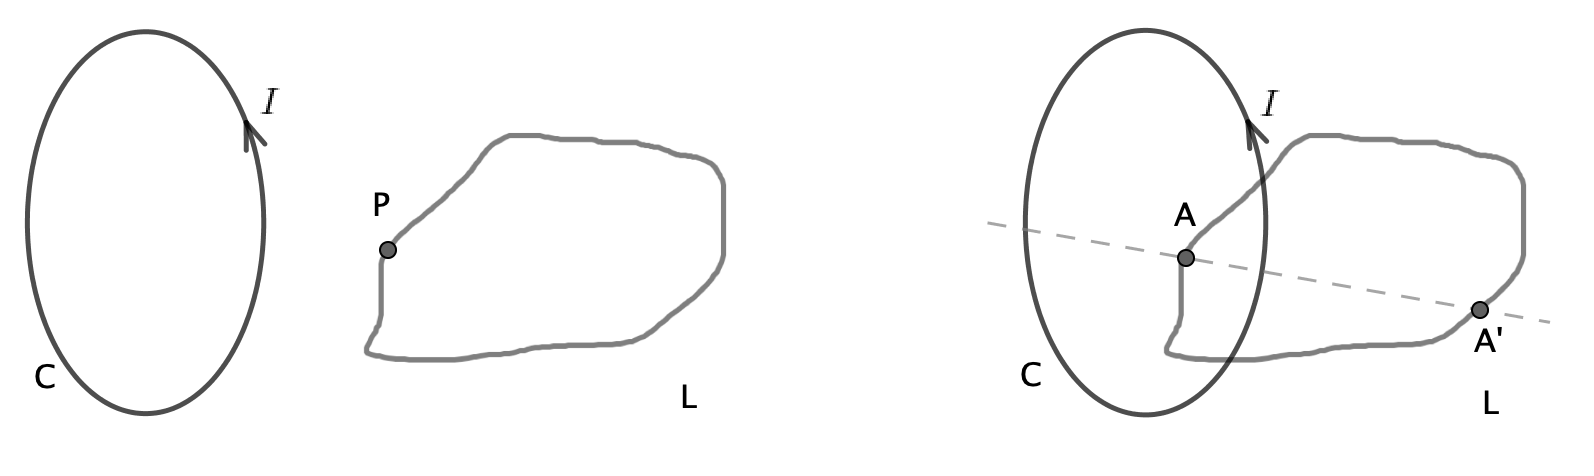
\includegraphics[width=.9\textwidth]{imagenes/imagenes27/T27IM03.png}
\end{figure}


--- L y C separados: $\ \Delta \Omega=0 \to \displaystyle \oint \vec B \cdot \dd \vec \lambda=0$

--- L y C unidos: Ángulo sólido inicial al subir hacia arriba en L es $\Omega1=2\pi$. En $A'$ vale $0$. Desde $A'$ hasta $A$ de nuevo, crece el ángulo sólido y cuando lleguemos a $A$ tendremos $2\pi$, pero como ha cambiado la simetría, $\Omega_2=-2\pi$. Luego,
$\ \Delta \Omega=\Omega_2-\Omega_1=-4\pi \to \displaystyle \oint \vec B \cdot \dd \vec \lambda = \mu_0 I$

Resumiendo, el th. de circulación de Ampère expresa que (si no se enlaza el circuito vale cero):
$\  \displaystyle \oint \vec B \cdot \dd \vec \lambda = \mu_0 I$. Si

Si lo que tenemos son $N$ circuitos enlazados, $\ I=\sum_i I_1$
\begin{multicols}{2}
Tomaremos como positivas aquellas cuyo sentido por la regla del sacacorchos coincida con el sentido de recorrido elegido en L

En el ejemplo de la imagen, $I=+I_1+I_2+I_1$, las tres son positivas y
se sustituye en $\  \displaystyle \oint \vec B \cdot \dd \vec \lambda = \mu_0 I$
\begin{figure}[H]
	\centering
	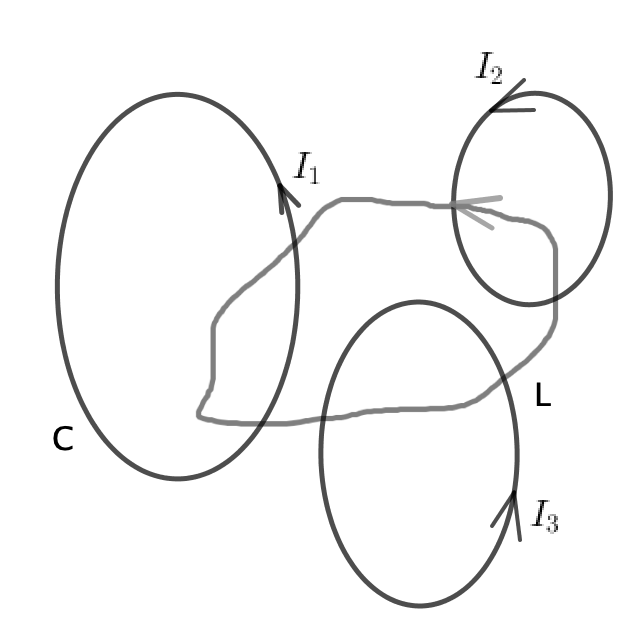
\includegraphics[width=.35\textwidth]{imagenes/imagenes27/T27IM04.png}
\end{figure}	
\end{multicols}

La ley de Ampère es útil en situaciones en las que el modelo del campo magnético tiene un alto grado de simetría. En tales situaciones, se usa la ley de Ampère para encontrar una relación entre el campo magnético como función de la posición y la corriente que genera el campo.

\textbf{Cálculo magnético en un conductor rectilíneo:}

\begin{multicols}{2}
Hay simetría.

El campo, en todo el circuito L ha de ser el mismo por la homogeneidad e isotropía del espacio.

Como están enlazados,

$ \displaystyle \oint \vec B \cdot \dd \vec \lambda = \mu_0 I$
\begin{figure}[H]
	\centering
	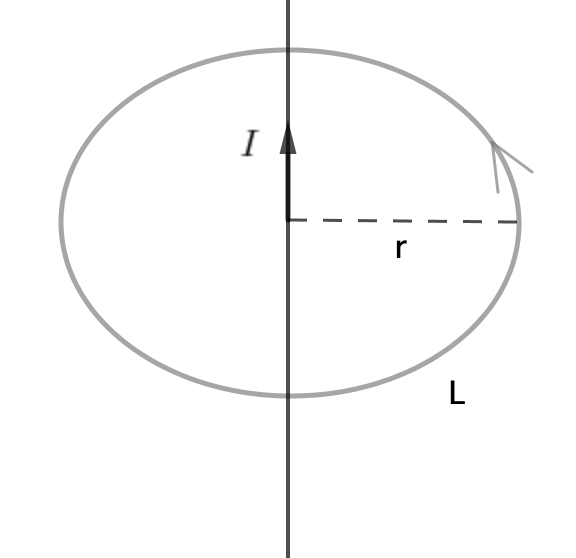
\includegraphics[width=.35\textwidth]{imagenes/imagenes27/T27IM05.png}
\end{figure}	
\end{multicols}

Si todos los puntos del circuito L tienen las mismas propiedades, en cualquier punto $\vec B \cdot \dd \vec \lambda$ ha de tomar el mismo valor. Esto solo ocurrirá si $\vec B$ es radial $(\theta=90^o)$ o $\vec B$ y $\dd \vec \lambda$ son paralelos $(\theta=0^o)$, con lo que 
	 $\vec B \cdot \dd \vec \lambda=B\dd \lambda$ y tendremos:
$\  \displaystyle \oint_L \vec B \cdot \dd \vec \lambda= \oint_L B \dd \lambda = B \ 2\pi r=\mu_0 I$

De donde, $\quad B=\dfrac{\mu_0 I}{2\pi r}\ $, $\quad$ que es la ley de Biot-Savart.

\textbf{Cálculo magnético en un conductor cilíndrico:}

Cilindro radio R por el que circula una intensidad I. La trayectoria elegida para calcular la circulación del campo serán circunferencias perpendiculares al cilindro conductor y de radio (distancia) $r$ al eje de éste. Como en el caso anterior, $\vec B \ || \dd \vec l$, con lo que $\oint \vec B \cot \dd \vec l=B\ 3\pi r = \mu_o \ I_{enc}$.

\vspace{5mm} %***********************************************
--- para $r<R,\ J=\dfrac I {\pi R^2 } \ \to I(r)=I_{enc}=J \pi r^2=I\dfrac{r^2}{R^2}$

$B\ 2\pi r=\mu_o \ I\dfrac{r^2}{R^2} \ \to B=\dfrac {\mu_o I}{2\pi} \dfrac{r^2}{R^2};\quad r<R$

\begin{multicols}{2}
--- para $r>R, \ B\ 2\pi r=\mu_o \ I_{enc}=\mu_o I \ \to \ B=\dfrac{\mu_0I}{2\pi r}\quad r>R$


Para $r>R$, es \emph{como si} toda la corriente estuviese concentrada a lo largo del eje del cilindro, como en el caso anterior de un conductor rectilíneo delgado. 
\begin{figure}[H]
	\centering
	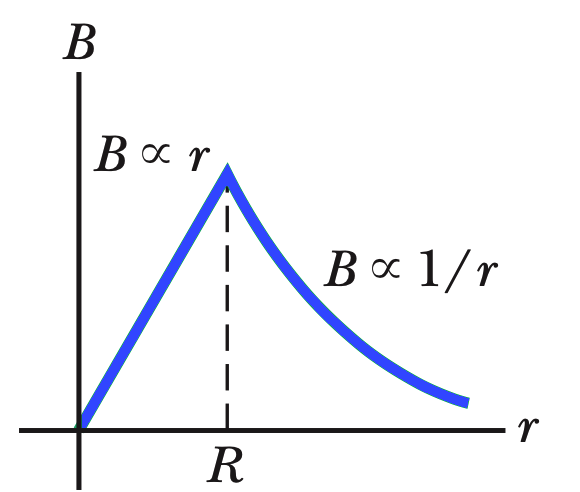
\includegraphics[width=.35\textwidth]{imagenes/imagenes27/T27IM07.png}
\end{figure}	
\end{multicols}

En capítulos anteriores vimos que la integral de línea del campo electrostático $\vec E$ alrededor de cualquier trayectoria cerrada es igual a cero, $\oint \vec E \dd \vec l =0$ ;  la fuerza electrostática  $\vec F = q \vec E$ sobre una carga $q$ es conservativa, también el campo electrostático es conservativo.

La fuerza magnética  $\vec F = q \vec v \times \vec  B$  sobre una partícula con carga en movimiento siempre es perpendicular a $\vec B$ , por lo que $\oint \vec B \cdot \dd \vec l$  se relaciona con la corriente total que cruza una superficie limitada por la trayectoria de integración. De hecho, la fuerza magnética sobre una partícula con carga en movimiento no es conservativa.  Una fuerza conservativa sólo depende de la posición del cuerpo sobre el que se ejerce la fuerza, pero la fuerza magnética sobre una partícula con carga y en movimiento también depende de la velocidad de la partícula. 

La ley de Ampère, como la hemos enunciado, resulta ser válida sólo si las corrientes son estables y si no están presentes magnéticos o campos eléctricos que varíen con el tiempo 

\begin{figure}[H]
	\centering
	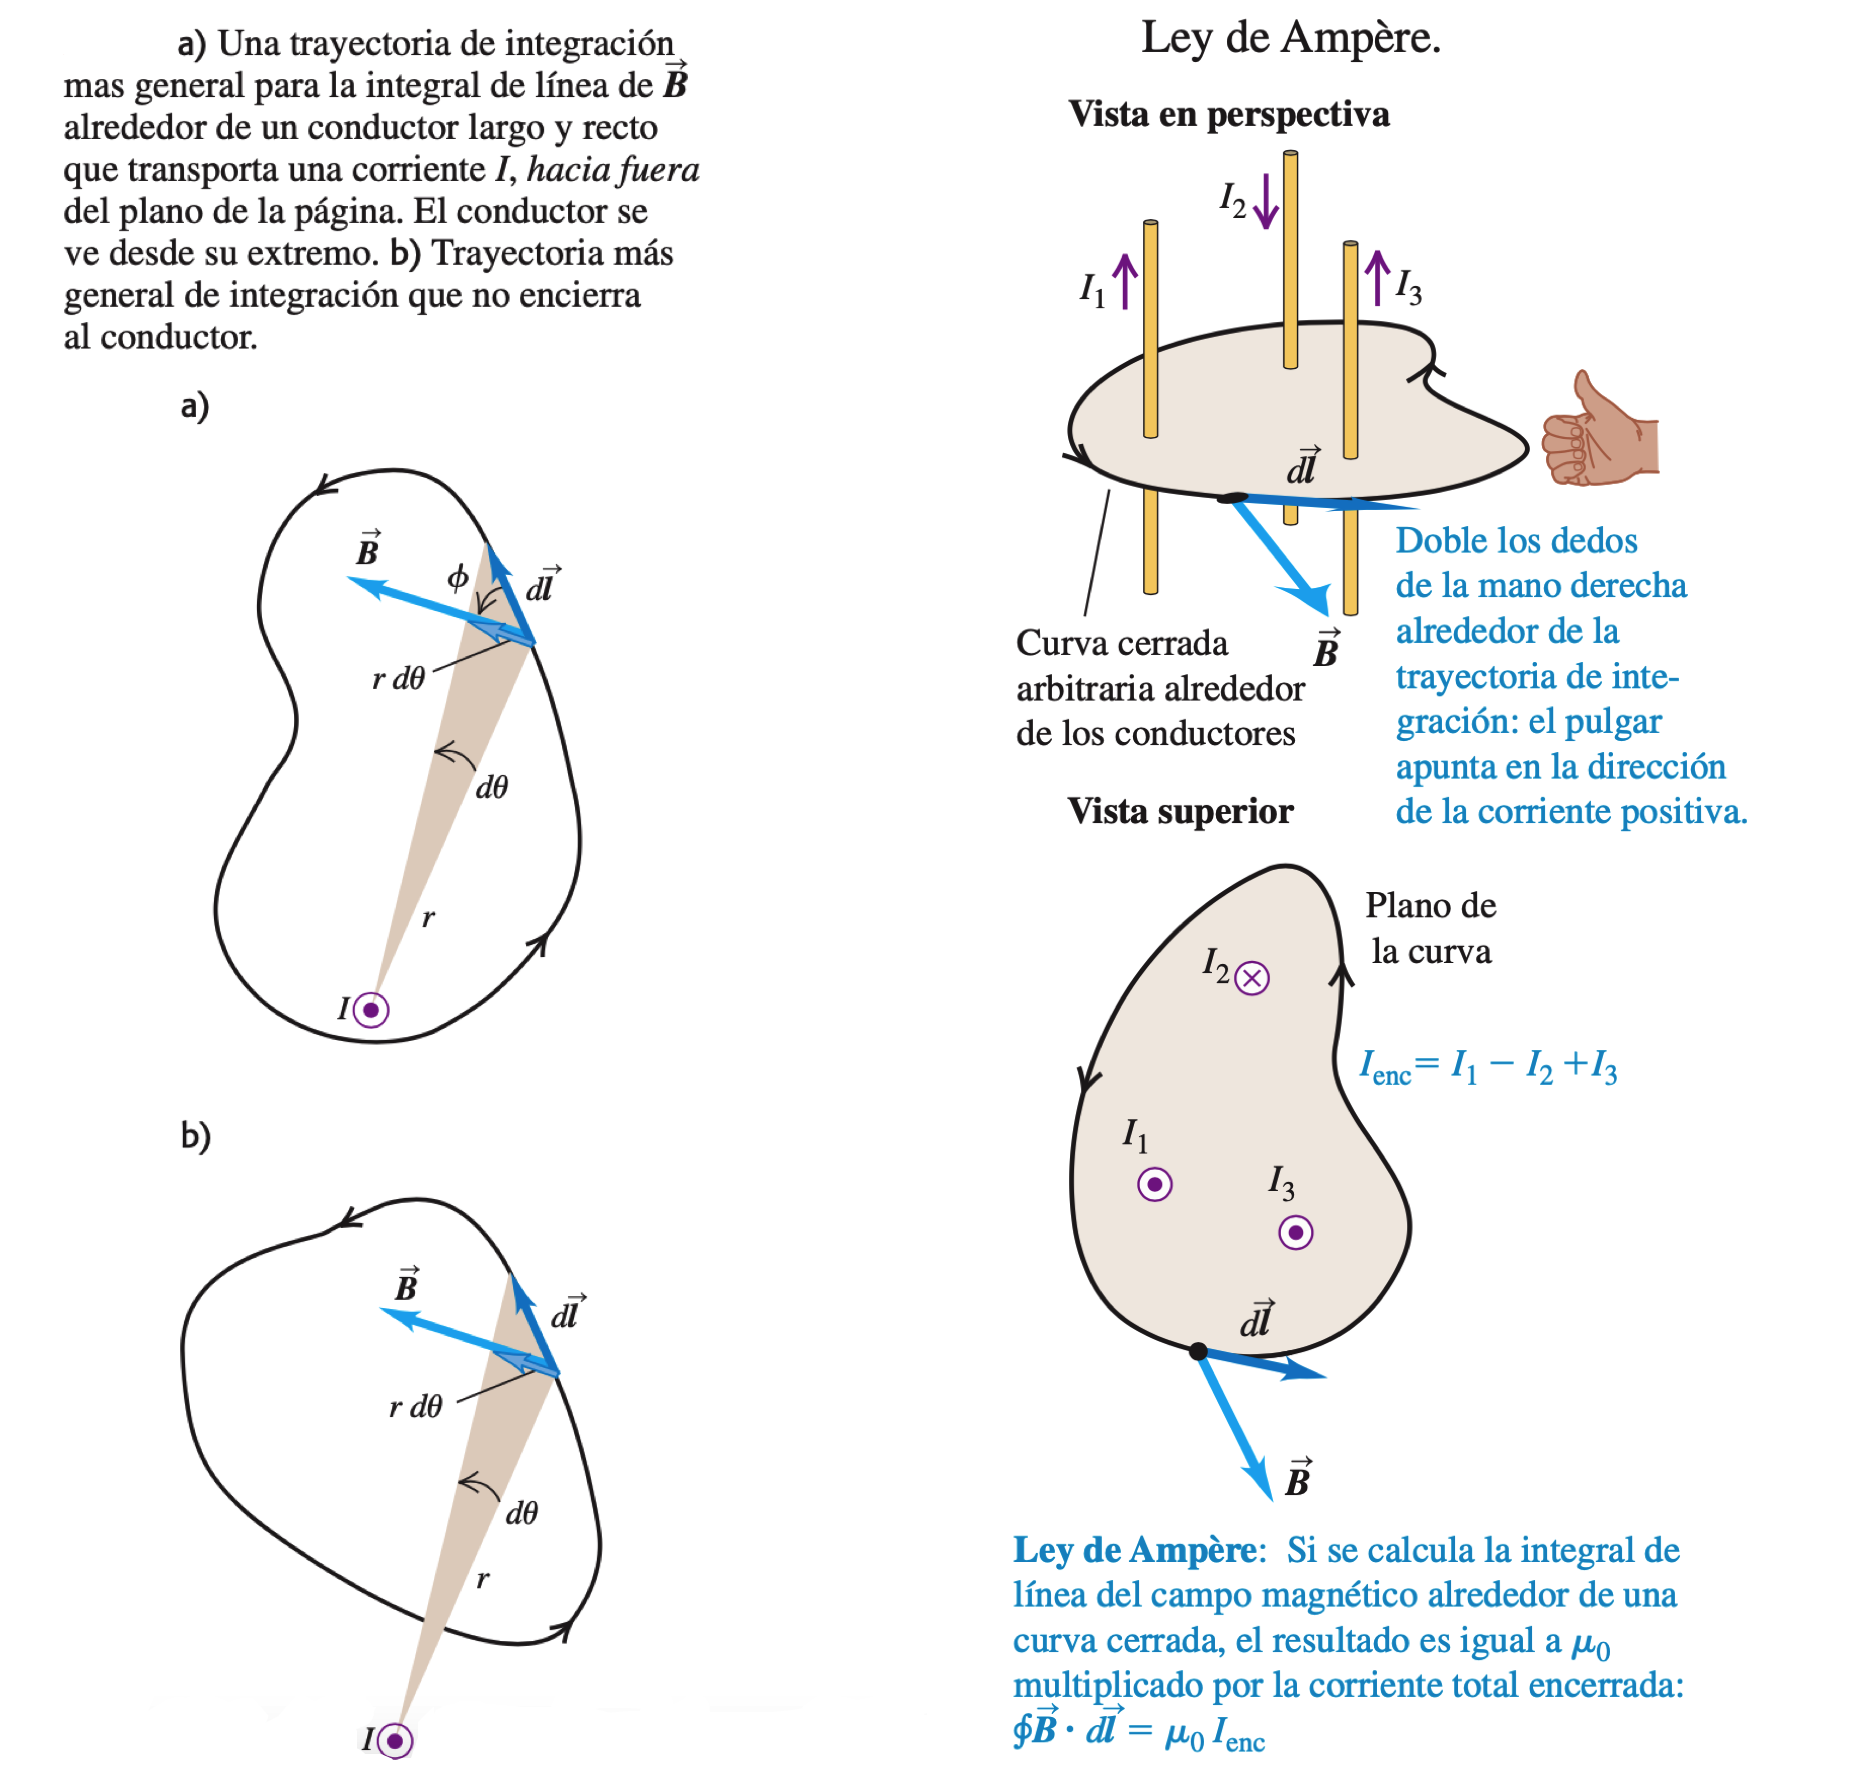
\includegraphics[width=1\textwidth]{imagenes/imagenes27/T27IM06.png}
\end{figure}


\section{Ley de Ampère en forma diferencial}

\begin{multicols}{2}
Para la ley de Gauss obtuvimos la siguiente relación local, 

$$ \vec \grad  \cdot \vec E = \dfrac{\rho}{\varepsilon_0}$$ 

Ahora, para el campo magnético, procederemos de forma análoga.


Circuito $PQRS$ contenido en el plano $YZ$.
\begin{figure}[H]
	\centering
	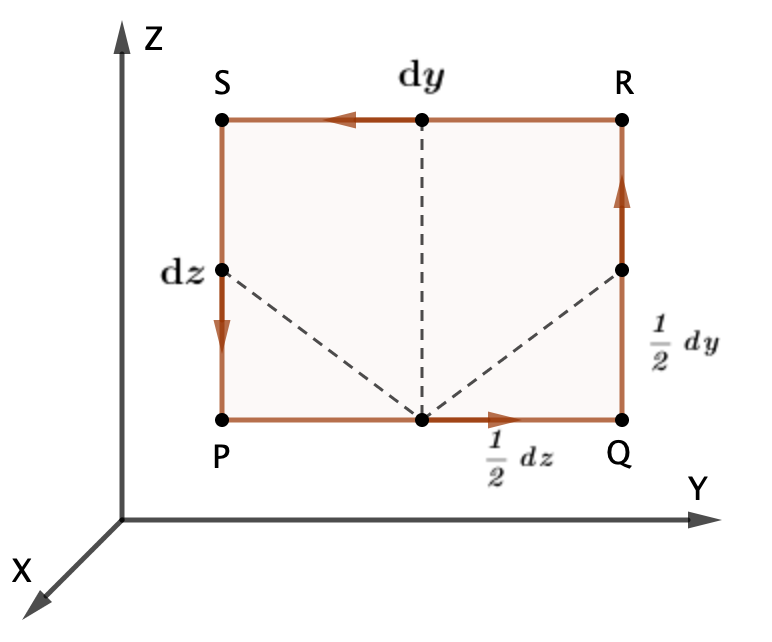
\includegraphics[width=.5\textwidth]{imagenes/imagenes27/T27IM08.png}
\end{figure}	
\end{multicols}

$(\vec B \cdot \dd \vec \lambda)_{PQRS}=(\vec B \cdot \dd \vec \lambda)_{PQ}+(\vec B \cdot \dd \vec \lambda)_{QR}+(\vec B \cdot \dd \vec \lambda)_{RS}+(\vec B \cdot \dd \vec \lambda)_{SP}$

Supongamos que en el punto $PQ$ hay un campo magnético $\vec B$; 

$(\vec B \cdot \dd \vec \lambda)_{PQ}=B_y \dd y$


$(\vec B \cdot \dd \vec \lambda)_{QR}=\displaystyle \left[ \vec B+\dfrac 1 2 \left( \pdv{\vec B}{y} \dd y + \pdv{\vec B}{z}  \dd z \right) \right]  \cdot \vec k \dd z$

$(\vec B \cdot \dd \vec \lambda)_{RS}=\displaystyle \left( \vec B+ \pdv{\vec B}{z} \dd z \right)   \cdot (-\vec j \dd y)$

$(\vec B \cdot \dd \vec \lambda)_{SP}=\displaystyle \left[ \vec B+\dfrac 1 2 \left( -\pdv{\vec B}{y} \dd y + \pdv{\vec B}{z}  \dd z \right) \right] \cdot (-\vec k \dd z)$

Luego, 

$(\vec B \cdot \dd \vec \lambda)_{PQ}=\displaystyle B_y \dd y$


$(\vec B \cdot \dd \vec \lambda)_{QR}=\displaystyle B_z \dd z +\dfrac 1 2 \left( \pdv {B_z}{y}\dd y + \pdv{B_z}{z} \dd z \right) \dd z$

$(\vec B \cdot \dd \vec \lambda)_{RS}=\displaystyle -B_y \dd y - \pdv{B_y}{z}\dd z \dd y $

$(\vec B \cdot \dd \vec \lambda)_{SP}=\displaystyle -B_z \dd z + \dfrac 1 2 \left( \pdv{B_z}{y} \dd y -\pdv{B_z}{z} \dd z \right) \dd z $

Sumando,

$\displaystyle (\vec B \cdot \dd \vec \lambda)_{PQRS}=\pdv{B_z}{y}\dd y \dd z - \pdv{By}{z}\dd z \dd y= \left( \pdv{B_z}{y} - \pdv{By}{z} \right)\ \dd y \ \dd z$

$\dd I = \vec J \cdot \dd \vec S= \vec J \cdot \left( \vec i \ \dd y \dd z \right) = J_x \ \dd y \dd z$

El teorema de Ampère asegura que $\displaystyle (\vec B \cdot \dd \vec \lambda)_{PQRS} =\mu_0 \dd I = \mu_o J_x \dd y \dd z$, es decir,
$\ \displaystyle  \pdv{B_z}{y} - \pdv{B_y}{z} = \mu_0 \ J_x$

Análogamente en los otros dos planos cartesianos.

$
\displaystyle  \pdv{B_z}{y} - \pdv{B_y}{z} = \mu_0 \ J_x; 
\qquad \displaystyle  \pdv{B_y}{x} - \pdv{B_x}{y} = \mu_0 \ J_y;
\qquad \displaystyle  \pdv{B_x}{z} - \pdv{B_z}{x} = \mu_0 \ J_z 	
$

En consecuencia,

\begin{equation}
\subrayado{ \ \boxed{ \ \boldsymbol{ \overrightarrow \grad \times \overrightarrow B \ = \ \mu_o \ \overrightarrow J } \ } \ } \qquad \textbf{Ley de Ampère en forma diferencial.}
\end{equation}

 Podemos usar esta ecuación para obtener el campo magnético cuando conocemos la distribución de corriente, y recíprocamente. En una región donde no haya corriente eléctrica, $\vec \nabla \times \vec B = \vec 0$.

La ley de Ampère en forma diferencial establece una relación local entre el campo magnético $\vec B$ en un punto y la densidad  de corriente $\vec J$ en el mismo punto del espacio, de un modo análogo a como la ley de Gauss relacionaba el campo eléctrico y la densidad de carga $\rho$ en el mismo punto del espacio.

\section{Flujo magnético}

Para todo campo vectorial se definen las \emph{líneas de campo} como aquellas curvas que son tangentes al valor del campo cada punto. En física, \emph{las líneas de campo} son una ayuda para visualizar un campo electrostático, magnético o cualquier otro campo vectorial estático. Esencialmente forman un mapa del campo 

Llamamos \emph{flujo del campo magnético} al número de líneas de campo que atraviesan una sección transversal a éste.

$$\boldsymbol{ \dd \Phi_B \ = } \ B \ \dd S_N= B \dd S \cos \theta \ \boldsymbol{ = \ \vec B \cdot \dd \vec S}$$

En el $SI$ de unidades, el flujo magnético se expresa en $\mathrm{T \ m}^{2} = \mathrm{Wb}$, weber\footnote{La unidad de flujo magnético recibe su nombre en honor al físico alemán Wilhelm Eduard Weber (1804-1891).}

Integrando para una superficie cerrada,

\begin{equation}
\subrayado{ \ \boldsymbol{ \Phi \ = \ \oint_S \vec B \cdot \dd \vec  S \ = \ 0} 	\ }
\end{equation}

Como no hay masas magnéticas o cargas magnéticas, en general, como no hay polos (o al menos no han sido observados), \emph{las líneas de fuerza del campo magnético $\vec B$ son cerradas}. Concluimos que
el flujo magnético a través de una superficie cerrada es siempre nulo. Esto es, el flujo entrante a través de cualquier superficie cerrada es igual al flujo saliente.

Por analogía con el campo eléctrico, $\Phi_B=\oint \vec B \cdot \dd \vec S = 0 \ \to \ \vec \nabla \cdot \vec B = 0$ que es la ley de Gauss para el campo magnético, \emph{``las líneas del campo magnético se cierran sobre sí mismas''}.

Conclusión,

\begin{equation}
\subrayado{ \ \boxed{ \ 
\boldsymbol{\vec \nabla \times \vec B \ = \ \mu_0 \ \vec J}
\ } \ }	
\qquad \qquad 
\subrayado{ \ \boxed{ \ 
\boldsymbol{\vec \nabla \cdot \vec B \ = \ 0 }
\ } \ }	
\end{equation}

\begin{figure}[H]
	\centering
	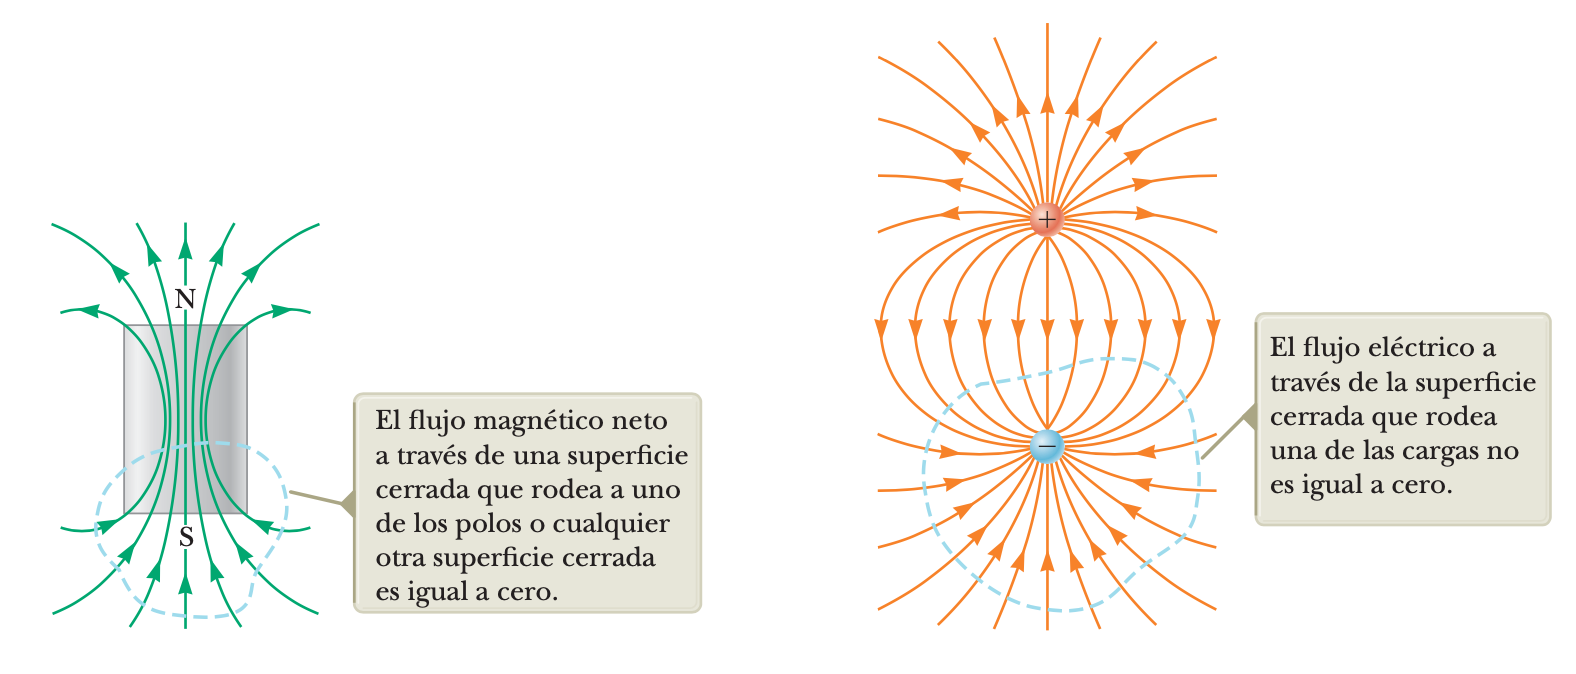
\includegraphics[width=1.05\textwidth]{imagenes/imagenes27/T27IM16.png}
\end{figure}















\section{Magnetización de la materia}


Dipolo magnético: $\ \vec M = I S \vec u_S$. La materia está constituida por átomos. El electrón $(-)$ órbita el núcleo atómico $(+)$. Este movimiento de cargas da lugar a una intensidad $I=Q/T$, donde $T$ es el periodo de revolución del electrón. Por lo visto en la interacción de los dos cuerpos, la órbita electrónica está contenida en un plano por lo que le podemos asociar un momento dipolar magnético: 
$\ \vec m = \dfrac e T \ S \ \vec u_S \ $

Ley de los cuerpos $\to$ tercera de Keppler $\to \ \dfrac{\dd S}{\dd t}=\dfrac 1 2 \dfrac L \mu \approx \dfrac 1 2 \dfrac L {m_e} = cte$

Integrando, $\ S=\dfrac 1 2 \dfrac {L T}{m_e}; \qquad \vec m = \dfrac e 2 \dfrac L {m_e}\ \vec u \quad \to \quad \vec m = - \dfrac{e}{2m_e} \vec L$

$\vec m = - \dfrac {e}{2m_e} \ I_{inercia} \ \vec \omega= - \dfrac 1 2 \ e \ r^2 \ \vec \omega\ ; \qquad \qquad \vec m = \vec m ( \vec \omega  )$

Tenemos una muestra de materia sometida a la acción de un campo magnético, todos los momentos magnéticos dipolares de todos los electrones se verán influídos por la presencia de ese campo magnético, se orientarán el la dirección de éste apareciendo así una dirección privilegiada, $\vec B$. El momento dipolar resultante será distinto de cero y se formará un imán. Para facilitar el cálculo supondremos una superficie cilíndrica.

\begin{figure}[H]
	\centering
	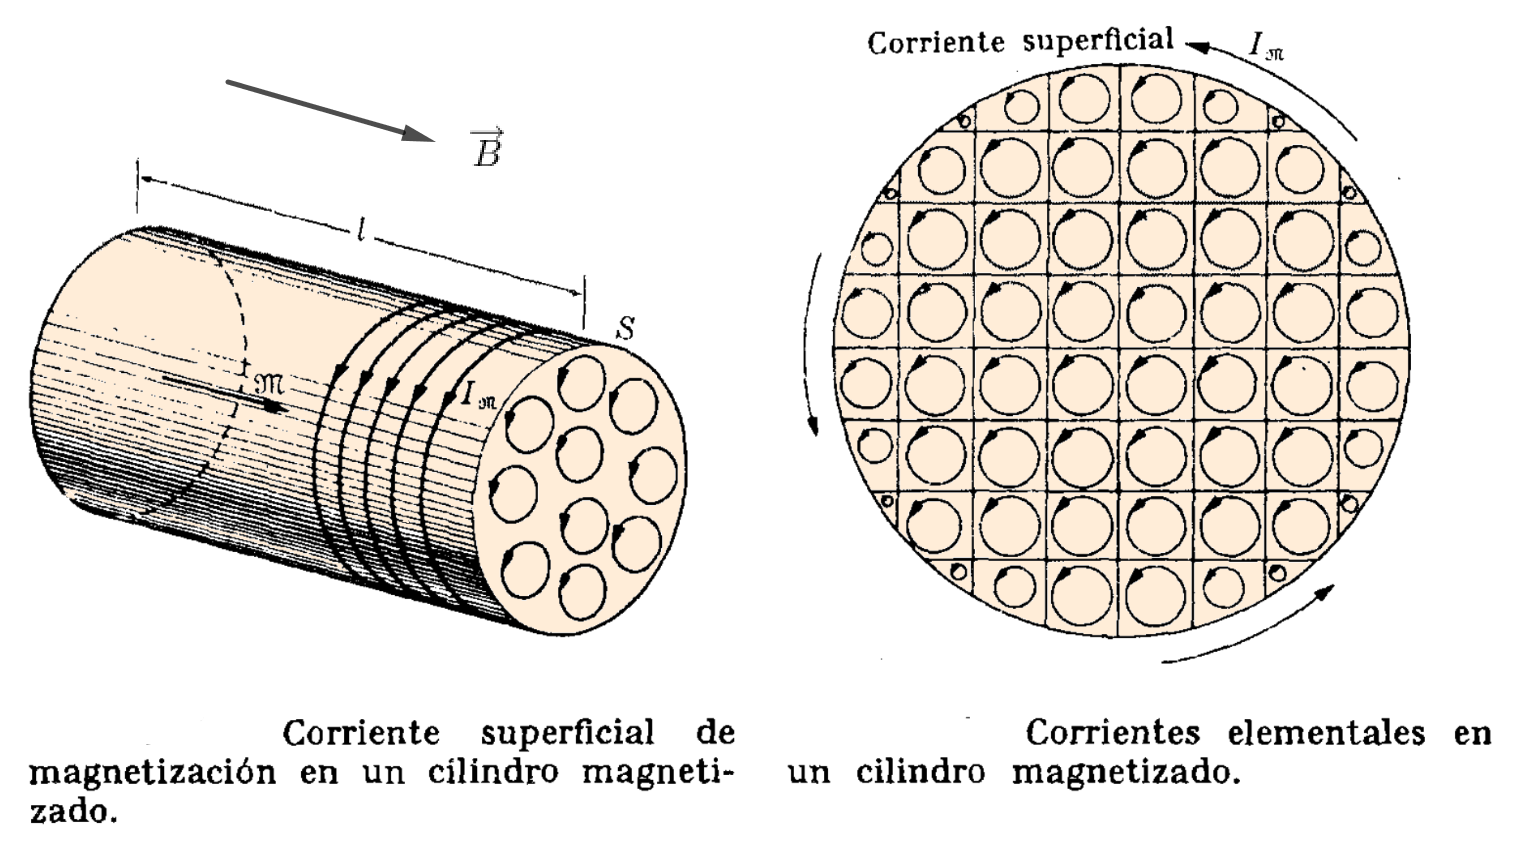
\includegraphics[width=1.05\textwidth]{imagenes/imagenes27/T27IM09.png}
\end{figure}	

Las corrientes en el interior del cilindro se anularán y solo quedarán  corriente en la superficie.
Como consecuencia se va a inducir una corriente superficial y decimos que el material se ha magnetizado y aparecen corrientes de magnetización  $I_M$.

Podemos asociar un vector de magnetización $\vec M$ que se define como el momento dipolar por unidad de superficie: $\displaystyle \vec M=\dv{\vec m}{\tau}$.

Si la muestra es homogénea, $n=$ número de átomos por unidad de volumen, $\vec M = n\ \vec m_i$, con $\vec m_i$ el momento dipolar magnético de cada una de las corrientes moleculares.

En el $SI$ de unidades, $[\vec M] \to \dfrac { \mathrm{A} \ \mathrm{m}^2 } {\mathrm {m}^3} = \mathrm{A\ m}^{-1}$

$\vec M = \dfrac{\dd \vec m}{\dd \tau}; \ \dd \vec m = \vec M \dd \tau$, si la muestra es homogénea, $\vec m_T=\vec M \ \tau$, en módulo,  $ m_T=M \ \tau$.

En nuestra muestra cilíndrica, $ m_T=M \ \tau = M\ LS$ que comparando con $m=IS$, tenemos

\begin{equation}
M\ L \ = \ I_M \qquad \text{corriente de magnetización} 	
\end{equation}


Aunque este resultado se ha obtenido para una disposición geométrica particular, es de validez general. De este modo podemos decir que
la corriente por unidad de longitud sobre la superficie de una porción de materia magnetizada es igual a la componente del vector magnetización $\vec M$ paralela al plano tangente a la superficie del cuerpo, y tiene dirección perpendicular a $\vec M$.
$\quad \vec M=\dfrac {I_M} L$, se mide en $\mathrm{A\ m}^{-1}$; $\quad \vec M \ || \ \vec S;\quad \vec M \ \bot \ S$

\section{Campo magnetizante}

Cuando la muestra es un conductor, que tiene cargas libres, aparece una intensidad debido a estas cargas libres que se mueven en el conductor, $I$ y también una intensidad de magnetización, $I_M$, debido a las corrientes congeladas.

Efectuemos la siguiente experiencia: enrollamos un solenoide a un conductor.

\begin{figure}[H]
	\centering
	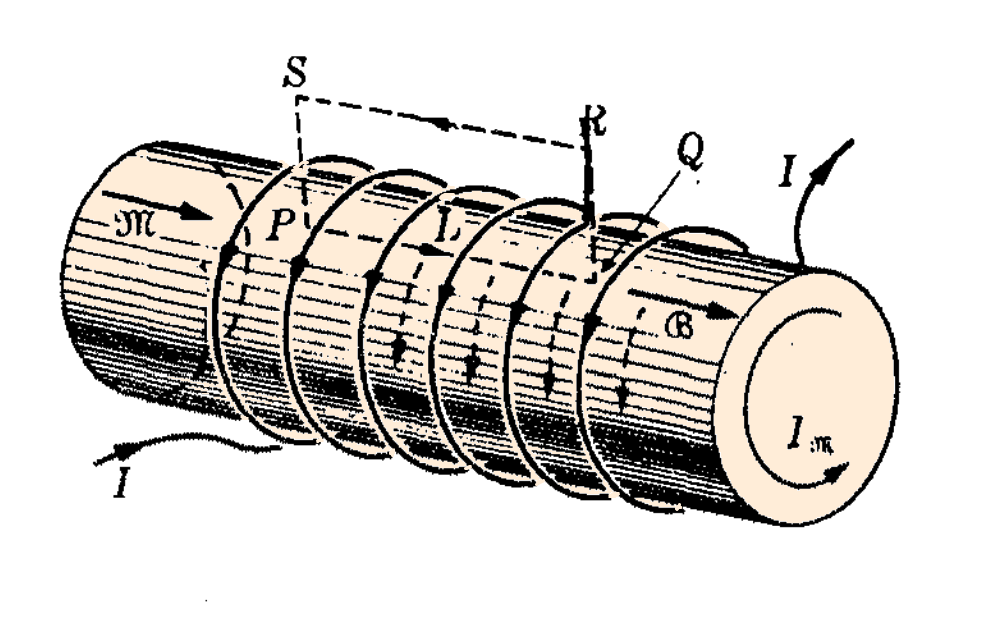
\includegraphics[width=0.95\textwidth]{imagenes/imagenes27/T27IM10.png}
\end{figure}

La muestra sometida a un campo magnético creado por el solenoide, se magnetiza. Podemos interpretarlo como un solenoide en el que $I_T=I_{\text{conductor}}+I_{\text{magnetización}}=I+I_M$

Vimos que el campo magnético creado por un solenoide es proporcional a la intensidad que circula por él.
$B=\mu_0 n I=\mu_0 \dfrac N L I$, donde debemos sustituir $I$ por la intensidad que en realidad fluye, $nI \to nI+M$, corriente por unidad de longitud que recorre la muestra.

$B=\mu_0 (nI+M) \ \to \ \dfrac B{\mu_0}-M=nI$, corriente por unidad de longitud.

Vectorialmente, $\ \boldsymbol{ \dfrac {\vec B}{\mu_0}-\vec M\ = \ \vec H } \ $, donde $\vec H$ es el \emph{campo magnetizante} o campo de excitación magnética.

Si multiplicamos la corriente por unidad de longitud por la longitud del solenoide tendremos la corriente: $HL=nIL$, es decir,

$\boldsymbol{HL\ =} \ nIL = I = \ \boldsymbol{I_{libre}}$, la asociada a la carga libre -electrones- capaces de moverse.

La circulación en $PQRS$ (ver figura anterior) será:

$| \overline{PQ} \ |=L; \qquad  \measuredangle(\vec H, \overrightarrow{QR}=90^o; \qquad  \vec H \times \overrightarrow{QR}=0$

$(\vec H \cdot \dd \vec \lambda)_{PQRS}=C_H=HL=I_{libre}$, por lo que

\begin{equation}
\boldsymbol{\oint_L \vec H \cdot \dd \vec \lambda \ = \ I_{libre}}	\qquad \text{Th. Ampére campo magnetizante}
\end{equation}


Como $\ \boldsymbol{ \dfrac {\vec B}{\mu_0}-\vec M\ = \ \vec H } \quad  \to \quad \vec B=\mu_0 \vec H +  \mu_0 \vec M $

Si no hay $\vec H$ no hay $\vec M$. Haciendo $\vec M = \chi_m \vec H$, con $\chi_m$ la \emph{constante de susceptibilidad magnética}, obtenemos:

$\vec B=\mu_0 (1+\chi_m) \vec M = \mu \vec M$

Se define la permeabilidad magnética relativa como $\mu'= \dfrac{\mu}{\mu_0}=1+\chi_m$, es una constante adimensional.

En todo material homogéneo ($\mu=cte$), $\displaystyle \vec B = \mu \vec H \ \to \ \oint_L \dfrac {\vec B}{\mu} \cdot \dd \vec \lambda = I_{libre}$

\begin{equation}
\subrayado{ \ \boxed{ \ \boldsymbol{
\oint \vec B \cdot \dd \vec \lambda \ = \ \mu \ I_{libre}
} \ } \ } 
\text{Th. Ampère	en presencia de material}
\end{equation}
 


Por ejemplo, el campo magnético de una corriente rectilínea dentro de un campo magnetizado es $B=\dfrac {\mu I}{2\pi r}$


\section{Problemas}

\begin{prob}
Se tiene dos barras de hierro idénticas, una imantada y la otra no. ?`Cómo saber cuál de las dos es un imán?	
\end{prob}

\begin{figure}[H]
	\centering
	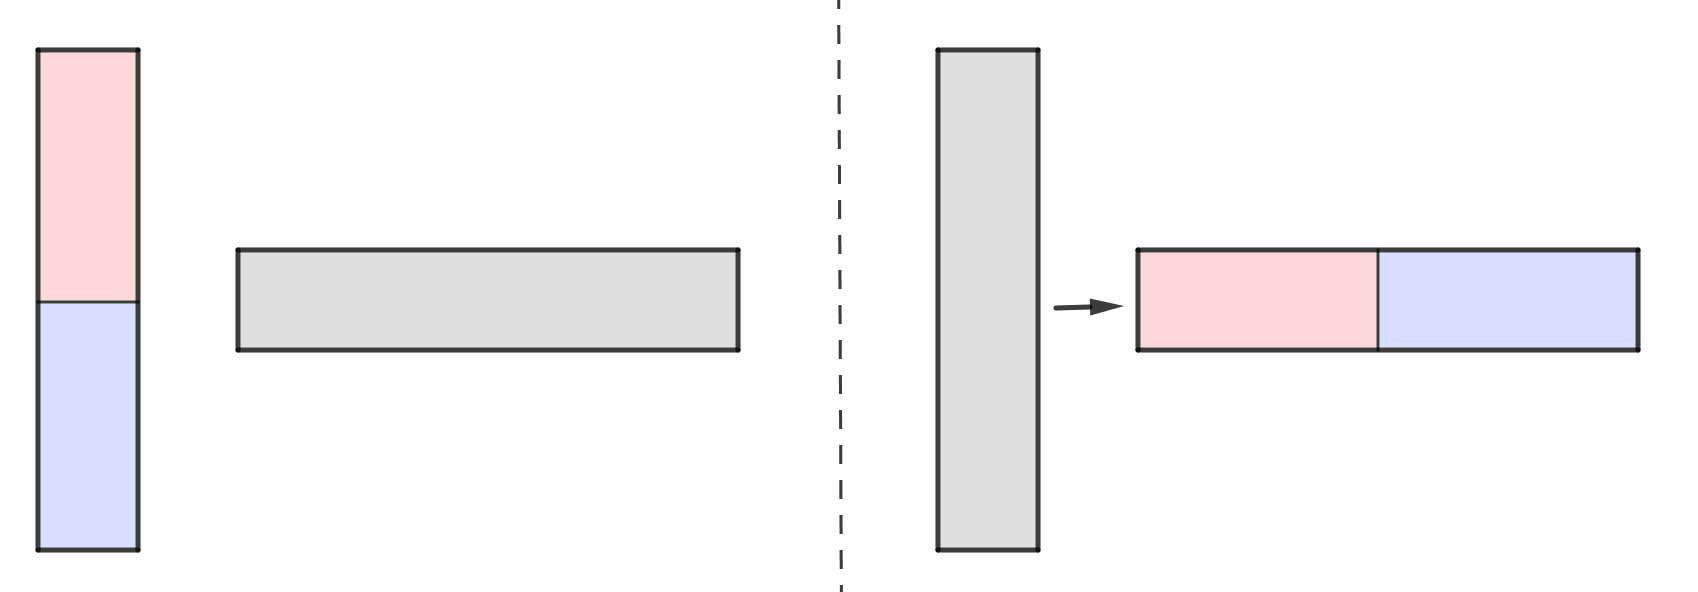
\includegraphics[width=0.75\textwidth]{imagenes/imagenes27/T27IM12.png}
\end{figure}

\vspace{20mm} %************************************


\begin{prob}
\begin{multicols}{2}
Una alambra largo de cobre lleva una intensidad de $10\ \mathrm{A}$. Calcular el flujo magnético por unidad de longitud de alambre para una superficie $S$ dentro del alambre, como se indica en la figura.	
\begin{figure}[H]
	\centering
	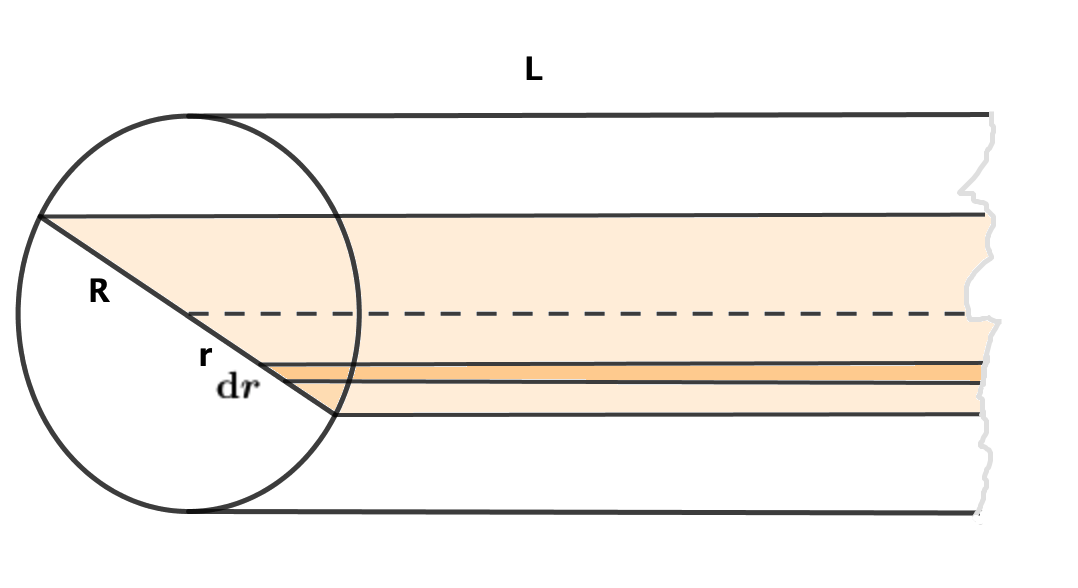
\includegraphics[width=0.5\textwidth]{imagenes/imagenes27/T27IM13.png}
\end{figure}
\end{multicols}
\end{prob}

$\dfrac I{\pi R^2}=\dfrac{I_{int}}{\pi r^2}$

Por th. Ampère: 

$\displaystyle \oint \vec B \cdot \dd \vec \lambda=\oint B \dd \lambda =B\oint \dd \lambda = B\ 2\pi r =\mu_o I_{int}=\mu_0 I \dfrac {r^2}{R^2} \ \to $ 

$B=\mu_0 \dfrac{Ir}{2\pi R^2}$

$\displaystyle \Phi_B=\int B \dd S = \dfrac{\mu_0 I}{2\pi R^2} \int_0^R
r \dd S =  \dfrac{\mu_0 I}{2\pi R^2} \int_=^R r L \dd r =  \dfrac{\mu_0 I}{2\pi R^2} L \dfrac {R^2}{2} =   \dfrac{\mu_0 I L}{4\pi}$

$\dfrac{\Phi_B}{L} \ = \  \dfrac{\mu_0 I}{4\pi} \ = \ 1=^{-6} \ \mathrm{Wb}$

\begin{prob}
Un disco de radio $R$	tiene una carga una carga $q$ uniformemente distribuida sobre su superficie y se le pone a girar con frecuencia angular $\omega$ sobre su eje. Determinar el campo magnético en el centro del disco y su momento magnético.
\end{prob}

\begin{multicols}{2}
	$B_{anillo}=\dfrac{\mu_o I}{2 r} \ \to \ \dd B=\dfrac{\mu_o \dd I}{2 a}=\dfrac{\mu_o}{2a} \dfrac {\dd q}{T}=\dfrac{\mu_0}{2a} \dfrac{\sigma \dd S}{2\pi / \omega}$
	
	$\displaystyle B= \int_0^R \dfrac{\mu_0 \omega \sigma}{4 \pi a} 2 \pi a \dd a = \dfrac{\mu_0 \omega q}{2\pi R}\ $ \textcolor{gris}{$(q=\sigma \pi R^2)$}
	\begin{figure}[H]
	\centering
	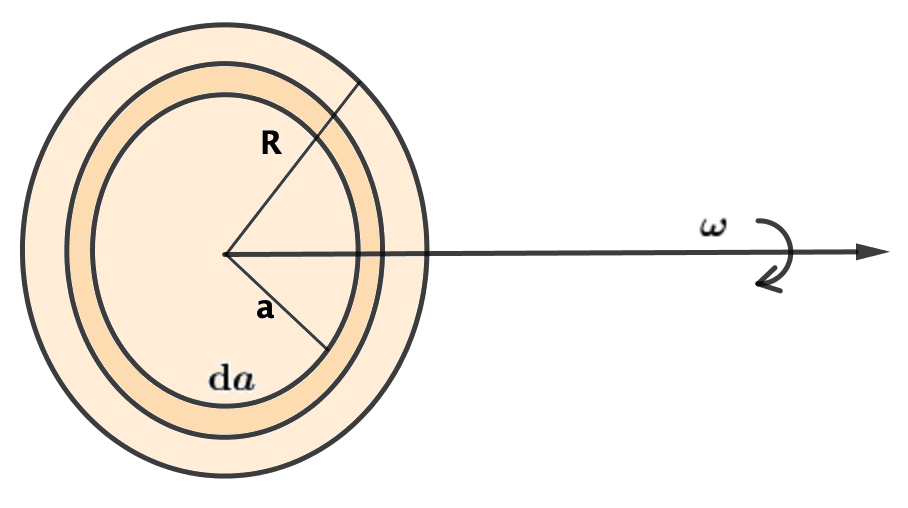
\includegraphics[width=0.5\textwidth]{imagenes/imagenes27/T27IM14.png}
\end{figure}
\end{multicols}

$\dd m=S\dd I=\pi a^2 \dd I=\pi a^2 \dfrac{\dd q}{T}=\pi a^2 \dfrac{\sigma \dd S}{2\pi /\omega}=\dfrac{\omega \sigma a^2}{2}2\pi a \dd a=\omega \sigma \pi a^3 \dd a$

$m=\dfrac{\omega \sigma \pi R^4}{4}=\dfrac{\omega \sigma (\pi R^2) R^2}{4}=\dfrac{\omega q R^2}{4}$

\begin{prob}.

\begin{multicols}{2}
Una espira rectangular de ancho $a$ y longitud $b$ se ubica cerca de un alambre largo que conduce una corriente $I$, como indica la figura adjunta. La distancia entre el alambre y el lado más cercano de la espira es $c$. El alambre es paralelo al lado largo de la espira. 

Encontrar el flujo magnético total a través de la espira debido a la corriente en el alambre.	
\begin{figure}[H]
	\centering
	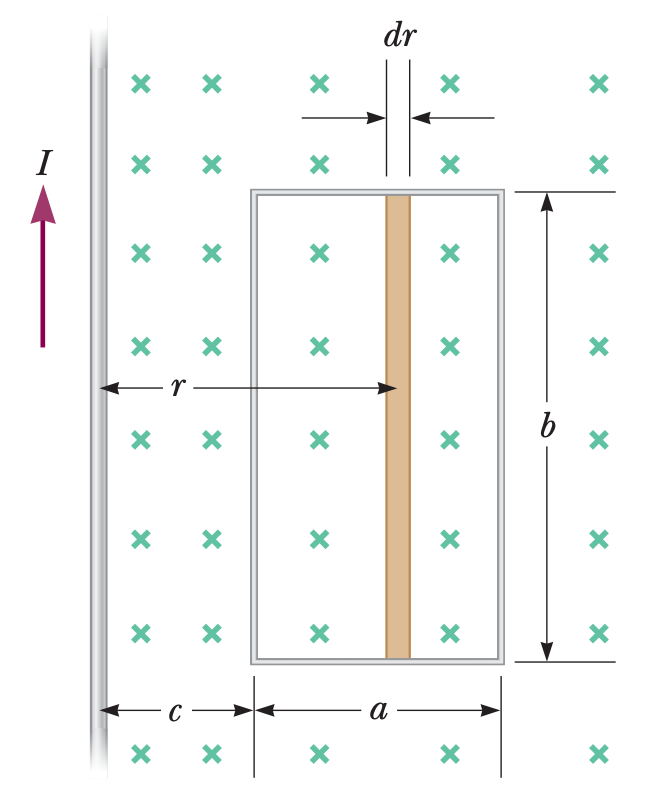
\includegraphics[width=0.45\textwidth]{imagenes/imagenes27/T27IM15.png}
\end{figure}
\end{multicols}
\end{prob}

$\vec B \ || \ \dd \vec S; \quad \dd S=b\dd r; \quad r\in[c,a+c]$

$\Phi_B=\displaystyle \int \vec B \cdot \dd \vec S = \int B \dd S =\int_c^{a+c} \dfrac {\mu_0 I}{2\pi r} b \dd r = \dfrac{\mu_0 Ib}{2 \pi} \int_c^{a+c} \dfrac{\dd r}{r}= \dfrac{\mu_0 Ib}{2 \pi} \left[ \eval{\ln r }_c^{a+c}  \right.$

$\Phi_B=\dfrac{\mu_0 Ib}{2 \pi} \ln \left( \dfrac{a+c}{a} \right) = \dfrac{\mu_0 Ib}{2 \pi} \ln \left( 1+\dfrac a c \right)$


Obsérvese como el flujo depende del tamaño de la espira. Incrementar $a$ o $b$ aumenta el flujo como era de  esperar. Si $c$ se vuelve tan grande tal que la espira esté muy alejada del alambre, el flujo tiende a cero, también como era de  esperar. \textcolor{gris}{Si $c$ tiende a cero, el flujo se vuelve infinito. En principio, este valor infinito se presenta porque el campo se vuelve infinito en $r = 0$ (si supone un alambre infinitamente delgado). Esto no ocurrirá en la realidad porque el grosor del alambre evita que el extremo izquierdo de la espira llegue a $r = 0$}.



\newpage %*****************************************************
\begin{myblock}{Imanes}
El imán es un cuerpo o dispositivo con un magnetismo significativo, de forma que atrae a otros imanes o metales ferromagnéticos (por ejemplo, hierro, cobalto, níquel y aleaciones de estos). 
\vspace{2mm} Tipos de imanes:
\begin{itemize}
\item Imanes naturales; la magnetita es un potente imán natural, tiene la propiedad de atraer todas las sustancias magnéticas. Su característica de atraer trozos de hierro es natural. Está compuesta por óxido de hierro. Las sustancias magnéticas son aquellas que son atraídas por la magnetita.

La magnetita es un mineral de hierro constituido por óxido ferroso-diférrico (Fe2+Fe3+2O4). Probablemente debe su nombre a la ciudad griega de Magnesia de Tesalia, en la actual prefectura de Magnesia. No obstante, una fábula de Plinio el Viejo atribuye el nombre al de un pastor de nombre Magnes que descubrió este mineral en el monte Ida, observando que se adhería a los clavos de su calzado

\item Imanes artificiales permanentes; las sustancias magnéticas que al frotarlas con la magnetita, se convierten en imanes, y conservan durante mucho tiempo su propiedad de atracción.
\item Imanes artificiales temporales; aquellos que producen un campo magnético solo cuando circula por ellos una corriente eléctrica. Un ejemplo es el electroimán.
\end{itemize}

\vspace{2mm} Oersted  evidenció en 1820 por primera vez que una corriente eléctrica genera un campo magnético a su alrededor. En el interior de la materia existen pequeñas corrientes relacionadas al movimiento de los electrones que contienen los átomos; cada una de ellas origina un microscópico imán. Cuando estos pequeños imanes están orientados en todas direcciones sus efectos se anulan mutuamente y el material no presenta propiedades magnéticas; y en cambio, si todos los imanes se alinean, actúan como un único imán y se dice que la sustancia se ha magnetizado.

\begin{figure}[H]
	\centering
	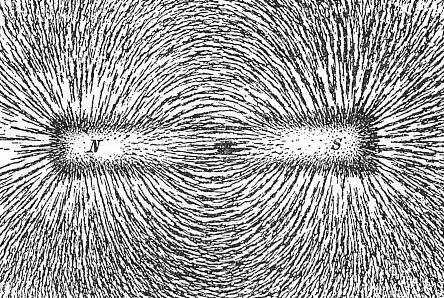
\includegraphics[width=0.9\textwidth]{imagenes/imagenes27/T27IM11.png}
\end{figure}

\vspace{2mm} Si se trata tanto de un tipo de imán como de otro, la máxima fuerza de atracción se halla en sus extremos, llamados polos. Un imán consta de dos polos, denominados polo norte y polo sur. Los polos iguales se repelen y los polos distintos se atraen. No existen polos aislados (monopolo magnético) y, por lo tanto, si un imán se rompe en dos partes, se forman dos nuevos imanes, cada uno con su polo norte y su polo sur, aunque la fuerza de atracción del imán disminuye.

\vspace{2mm} Entre ambos polos se crean líneas de fuerza, siendo estas líneas cerradas, por lo que en el interior del imán también van de un polo al otro. Como se muestra en la figura, pueden ser visualizadas esparciendo limaduras de hierro sobre una cartulina situada encima de una barra imantada; golpeando suavemente la cartulina, las limaduras se orientan en la dirección de las líneas de fuerza.

\end{myblock}

